\documentclass[11pt,a4paper]{article}
\usepackage[top=3cm, bottom=2cm, left=3cm, right=2cm]{geometry}
\usepackage[utf8]{inputenc}
% \usepackage[T1]{fontenc}
\usepackage{amsmath, amsfonts, amssymb}
\usepackage{siunitx}
\usepackage[brazil]{babel}
\usepackage{graphicx}
\usepackage[margin=10pt,font={small, it},labelfont=bf, textfont=it]{caption}
\usepackage[dvipsnames, svgnames]{xcolor}
\DeclareCaptionFont{MediumOrchid}{\color[svgnames]{MediumOrchid}}
\usepackage[pdftex]{hyperref}
\usepackage{natbib}
\bibliographystyle{plainnat}
\bibpunct{[}{]}{,}{s}{}{}
\usepackage{color}
\usepackage{footnote}
\usepackage{setspace}
\usepackage{booktabs}
\usepackage{multirow}
\usepackage{subfigure}
\usepackage{fancyhdr}
\usepackage{leading}
\usepackage{indentfirst}
\usepackage{wrapfig}
\usepackage{mdframed}
\usepackage{etoolbox}
\usepackage[version=4]{mhchem}
\usepackage{enumitem}
\usepackage{caption}
\DeclareCaptionLabelFormat{figuras}{\textcolor{CarnationPink}{Figura \arabic{figure}}}
\captionsetup[figure]{labelformat=figuras}

\makeatletter
\renewcommand\tagform@[1]{\maketag@@@{\color{CarnationPink}(#1)}}
\makeatother

\renewcommand{\theequation}{Eq. \arabic{equation}}
\renewcommand{\thefigure}{Fig. \arabic{figure}}

\setlist[itemize]{label=\textcolor{CarnationPink}{$\mathbf{\square}$}}

\setlist[enumerate]{label=\textcolor{CarnationPink}{\arabic*.}, align=left}


\newcounter{exemplo}

\NewDocumentEnvironment{exemplo}{ O{} }{%
\allowbreak
\setlength{\parindent}{0pt}
  \begin{mdframed}[
  leftline=true,
  topline=false,
  rightline=false,
  bottomline=false,
  linewidth=2pt,
  linecolor=CarnationPink,
  frametitlerule=false,
  frametitlefont=\Large\bfseries\color{CarnationPink},
  frametitle={\color{CarnationPink}\normalfont\bfseries #1},
  ]
}{%
  \end{mdframed}
}

\setlength{\fboxsep}{10pt}
\setlength{\fboxrule}{1pt}
\usepackage{float}
\renewcommand{\thefootnote}{\alph{footnote}}
\usepackage{url}
\hypersetup{
    colorlinks=true,
    linkcolor=cyan,
    filecolor=cyan,      
    urlcolor=cyan,
    citecolor=cyan,
    pdftitle={Resumos}
}
\pagestyle{fancy}
\fancyhf{}
\renewcommand{\headrulewidth}{0pt}
\rfoot{Página \thepage}

\title{Dosimetria}
\author{Dosimetria de Referência\nocite{*}}
\date{\textit{Dalila Mendonça}}
\begin{document}
	\maketitle

    \section{Introdução}

    A finalidade da dosimetria é determinar a dose absoluta entregue.  O principal instrumento utilizado para este fim são as câmaras de ionização e a dose absorvida é dada pela medida da ionização no meio que é convertida para a dose absorvida por meio de um fator de calibração fornecido por um laboratório de calibração credenciado.

    O fator de calibração pode ser dado diretamente em termos da dose absorvida na água para feixes de MV ou em termos do Kerma no ar, para fótons kV e fontes de braquiterapia.

    O padrão para a dose absorvida é definido pelo Laboratório Padrão Primário, que fornece o fator de calibração para o laboratório padrão secundário (laboratório credenciado) que é então responsável por fornecer o fator de calibração para o usuário final.

    O padrão é que os laboratórios façam a calibração para uma qualidade de feixe do \ce{^{60}Co}, embora alguns laboratórios (o que não é o caso do Brasil) possuem outras qualidades disponíveis, sendo possível fornecer o fator de calibração para diferentes qualidades de feixe. 

    Para fatores de calibração determinados para qualidades de feixes diferente da qualidade que está sendo calibrada, é necessário aplicar um fator de correção para adequar o fator de calibração para a qualidade de interesse.

	\section{Definições}

  		\begin{itemize}
			\item \textcolor{CarnationPink}{Instrumento de referência}: Instrumento calibrado por um laboratório padrão e utilizado para a calibração do feixe do usuário.
			\item \textcolor{CarnationPink}{Instrumento de campo}: Instrumento calibrado via calibração cruzada com um instrumento de referência e normalmente utilizado em medidas rotineiras;
		\end{itemize}

	\section{Formalismo do $N_{D,w}$}

	\subsection{Formalismo}

	A dose absorvida na água em uma profundidade $z_{ref}$ na água para um feixe de referência com qualidade $Q_0$ e na ausência da câmara é dado por:

  		\begin{equation}
			D_{w,Q_0} = M_{Q_0} \; N_{D,w,Q_{0}}
		\end{equation}
  		

  		\begin{exemplo}[onde:]
			\begin{itemize}[label=\textcolor{CarnationPink}{$\star$}]
				\item \textbf{\textcolor{CarnationPink}{$\mathbf{D_{w,Q_0}}$}} é a dose absorvida na água na profundidade de referência;
				\item \textbf{\textcolor{CarnationPink}{$\mathbf{M_{Q_0}}$}} é a leitura do dosímetro sob as condições de referência utilizadas nos laboratórios credenciados;
				\item \textbf{\textcolor{CarnationPink}{$\mathbf{N_{D,w,Q_{0}}}$}} é o fator de calibração  do dosímetro em termos da dose absorvida na água fornecido pelo laboratório padrão.
			\end{itemize}
		\end{exemplo}

	As medidas deverão ser realizadas sob as mesmas condições de referência utilizadas durante a calibração, e aquelas que não são possíveis ser alcançadas, são chamadas de quantidades de influência, e precisam ser corrigidas por fatores de correção para adequar a leitura da câmara com o fator de calibração que será utilizado para determinar a dose absorvida na água.

	Quando a câmara é utilizada para calibrar um feixe com uma qualidade diferente daquela que ele foi calibrado, é necessário corrigir a o fator de calibração para a qualidade do feixe no qual o dosímetro será utilizado. Este fator é chamado de Fator de Correção de Qualidade.

	\subsection{Fator de Correção para a Qualidade do Feixe}

	Quando um dosímetro é utilizado em uma qualidade de feixe $Q$ diferente daquela utilizada para determinar o fator de calibração $Q_0$, a dose absorvida na água é dada por:

		\begin{equation}
			D_{w,Q} = M_Q \; N_{D,w,Q_0} \; k_{Q,Q_0}
			\label{eq:doseAguaCorrigidaQualidade}
		\end{equation}

		\begin{exemplo}[onde:]
			\begin{itemize}[label=\textcolor{CarnationPink}{$\star$}]
				\item \textbf{\textcolor{CarnationPink}{$\mathbf{k_{Q,Q_0}}$}} é o fator que corrige os efeitos da diferença entre a qualidade do feixe de referência $Q_0$ e a qualidade do feixe sendo calibrado pelo usuário $Q$; e
				\item \textbf{\textcolor{CarnationPink}{$\mathbf{M_Q}$}} é a leitura do dosímetro para a qualidade $Q$ corrigida pelos valores de referência das quantidades de influência, como pressão, temperatura, polaridade, recombinação iônica e humidade;
			\end{itemize}
		\end{exemplo}

		O fator de calibração da qualidade $k_{Q,Q_0}$ é definido como a razão do fator de calibração para a qualidade $Q$ a ser calibrada pelo fator de calibração para a qualidade de referência, ou seja:

			\begin{equation}
				k_{Q,Q_0} = \frac{N_{D,w,Q}}{N_{D,w,Q_0}} = \frac{D_{w,Q}/M_Q}{D_{w,Q_0}/M_{Q_0}}
			\end{equation}

		Quando o feixe de referência é o \ce{^{60}Co}, $k_{Q,Q_0} = k_Q$ para fins de simplificação.  O ideal é que o fator de qualidade do feixe fosse medido para cada câmara, para cada qualidade de feixe utilizada pelo usuário. Porém seria necessário que o laboratório tivesse acesso às qualidades do feixe apropriada e portanto é restrito a apenas alguns laboratórios padrão primário.

		Caso não houver dados experimentais disponíveis ou caso não seja possível medir diretamente o $k_{Q,Q_0}$, ele pode ser determinado teoricamente através da aplicação da teoria cavitária de Bragg-Gray, de modo que:

			\begin{equation}
				K_{Q,Q_0} = \frac{(s_{w,ar})_Q}{(s_{w,ar})_{Q_0}} \; \frac{(W_{ar})_{Q}}{(W_{ar})_{Q_0}} \; \frac{p_{Q}}{p_{Q_0}}
				\label{eq:kqqBraggGray}
			\end{equation}

			\begin{exemplo}[onde:]
				\begin{itemize}[label=\textcolor{CarnationPink}{$\star$}]
					\item \textbf{\textcolor{CarnationPink}{$\mathbf{s_{w,ar}}$}} é a razão entree poder de freamento de Spencer/Attix (restrito) da água e do ar para as qualidades $Q$ e $Q_0$;
					\item  \textbf{\textcolor{CarnationPink}{$\mathbf{W_{ar}}$}} é a energia média para formar um par de íons no ar para a qualidades $Q$ e $Q_0$;
					\item \textbf{\textcolor{CarnationPink}{$\mathbf{p}$}} considera todos os fatores de perturbação que consideram todos os desvios para as condições ideais da cavidade de Bragg-gray (parede, eletrodo, cavidade, etc\dots);
				\end{itemize}
			\end{exemplo}

		Esta  é valida para todos tipos de feixes de alta energia. Em feixes terapeuticos de fótons e elétrons pode-se assumir que $(W_{ar})_{Q} = (W_{ar})_{Q_0}$ de modo que :
		
			\begin{equation}
				K_{Q,Q_0} \approx  \frac{(s_{w,ar})_Q}{(s_{w,ar})_{Q_0}} \; \frac{p_{Q}}{p_{Q_0}}
				\label{eq:kqqAproximacao}
			\end{equation}

		Os únicos fatores que são específicos da câmara são os fatores de correção de perturbação. o TRS-398 fornece os valores do produto $(s_{w,ar})_{Q_0} \cdot p_{Q_0}$ para diversas câmaras cilíndricas em seu apendice B.

		Em casos de feixes de baixa e média energia, a \ref{eq:kqqBraggGray} não pode ser utilizada porque essas energias não se aplicam às condições da teoria de Bragg-Gray além da respostas das câmaras variarem de uma para a outra nessas energias; Portanto, nesse caso, o formalismo do TRS-398 é baseado exclusivamente nas medidas diretas do $N_{D,w,Q}$ ou do $K_{Q,Q_0}$.

	\subsection{$K_{Q,Q_0}$ para Calibração Cruzada de feixes de elétrons}

		Para dosímetros que serão utilizados para dosimetria de feixe de elétrons, existem três possibilidades para sua calibração:

		\begin{enumerate}
			\item Para dosímetros utilizados em feixes de elétrons que foram calibrados na qualidade do feixe de \ce{^{60}Co}, o fator $K_{Q,Q_0}$ é dado pela \ref{eq:kqqBraggGray}. 
			
			\item Determinar o fator de calibração da câmara diretamente no feixe de elétrons, o que é limitado devido à disponibilidade em oferecer essas calibrações. Caso possível, uma opção seria fornecer o $K_{Q,Q_0}$ para as diferentes qualidades de feixes de elétrons utilizadas pelo usuário;
			
			\item Realizar a calibração cruzada de uma câmara de placas paralelas em comparação com uma câmara de ionização cilíndrica calibrada em um feixe de elétrons de alta energia com qualidade $Q{cross}$. 
		\end{enumerate}

		O fator $K_{Q,Q_{cross}}$ determinado para a câmara de placas paralelas irá permitir o uso da câmara de para um feixe de elétrons com qualidade Q, porém a determinação do $K_{Q,Q_{cross}}$ não é trivial porque a qualidade de calibração cruzada $Q{cross}$ não é única e, portanto, para cada tipo de câmara, será necessária uma tabela bidimensional de fatores $K_{Q,Q_{cross}}$.

		Porém, é possível apresentar os dados necessários em uma única tabela, introduzindo uma qualidade arbitrária de feixe de elétrons ($Q_{int}$) que atua como uma qualidade intermediária entre a qualidade de calibração cruzada ($Q{cross}$) e a qualidade do usuário ($Q$). $Q_{int}$ é apenas uma ferramenta para apresentação dos dados e nenhuma medida em $Q_{int}$ precisa ser realizada. 

		O fator $K_{Q,Q_{cross}}$ é determinado como a razão entre os fatores $K_{Q,Q_{int}}$ e $K_{Q_{cross},Q_{int}}$, ou seja:

			\begin{equation}
				k_{Q,Q_{cross}} = \frac{K_{Q,Q_{int}}}{K_{Q_{cross},Q_{int}}}
				\label{eq:kqqcross}
			\end{equation}

		O fator $(K_{Q_{cross},Q_{int}})^{-1}$ corrige o fator de calibração da câmara atual $N_{D,w,Q_{cross}}$ em um fator de calibração que se aplica a qualidade intermediária $Q_{int}$ e o fator $K_{Q,Q_{int}}$ corrige o fator de calibração para a qualidade intermediária para o fator de calibração para a qualidade $Q$ e então a  \ref{eq:doseAguaCorrigidaQualidade} pode ser aplicada para determinar a dose na água.

		Aplicando a \ref{eq:kqqAproximacao} em  $K_{Q_{cross},Q_{int}}$ e $K_{Q,Q_{int}}$, a razão entre os fatores de perturbação e entre os poderes de freamento para $Q_{int}$ na \ref{eq:kqqcross} irão se cancelar e portanto, $Q_{int}$ pode ser escolhida de forma arbitrária. O TRS-398 adota para $Q_{int}$ a qualidade $R_{50} = 7.5 \; g \; cm^{-2}$, onde $R_{50}$ é o índice de qualidade para feixe de elétrons. Os valores para $K_{Q_{cross},Q_{int}}$ e para  $K_{Q,Q_{int}}$ com base nessa qualidade intermediária são podem ser encontrados na tabela 7.IV (\ref{fig:tabela74trs398}) do TRS-398. Os valores de $K_Q$ para feixes de elétrons para as câmaras de ionização calibradas em feixes de \ce{^{60}Co} são obtidos na tabela 7.III (\ref{fig:tabela73trs398}).

		\begin{figure}[h]
			\centering
			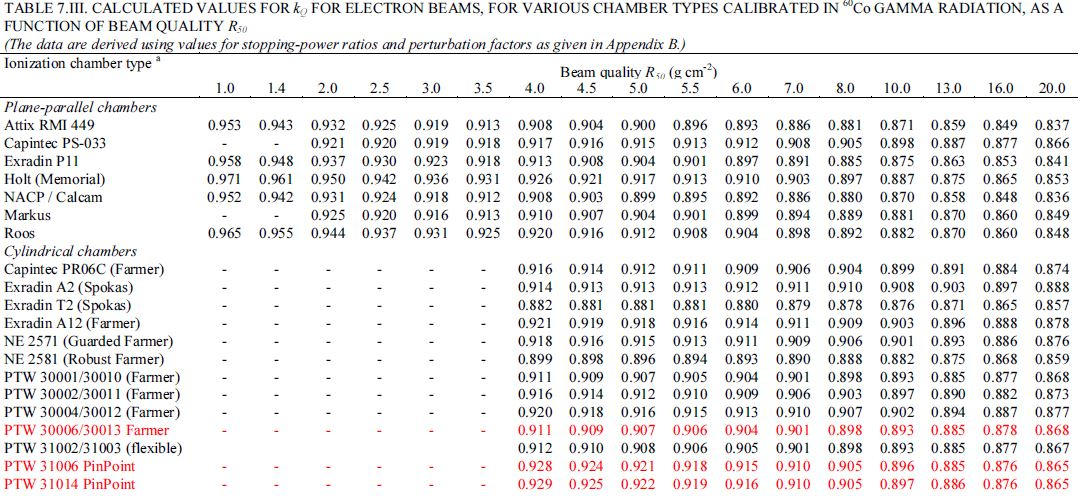
\includegraphics[width=0.9\textwidth]{Imagens/tabela73trs398.JPG}
			\caption{Valores calculados para o $K_Q$ para as câmaras de ionização calibradas em feixes de \ce{^{60}Co} }
			\label{fig:tabela73trs398}
		\end{figure}

		\begin{figure}[h]
			\centering
			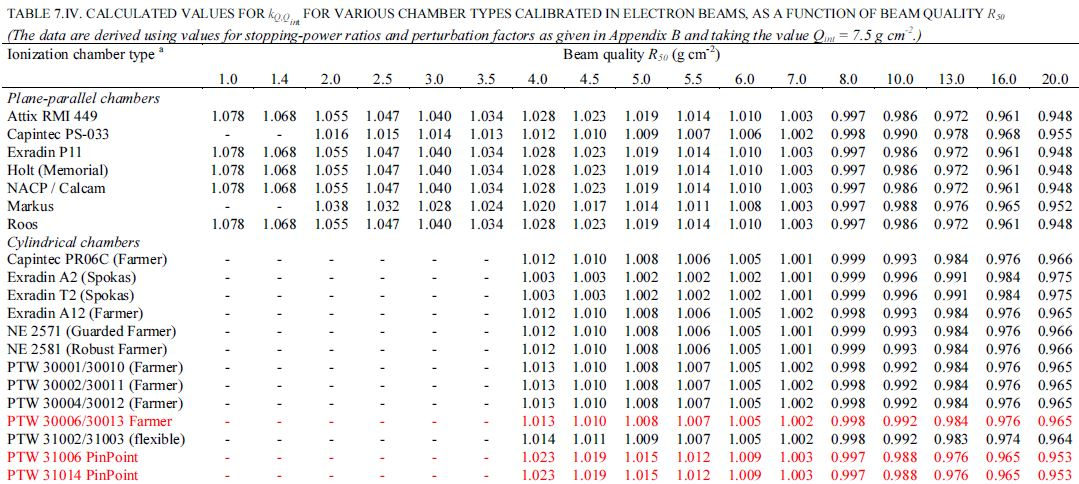
\includegraphics[width=0.9\textwidth]{Imagens/tabela74trs398.JPG}
			\caption{Valores calculados para o $K_{Q,Q_{int}}$ em função do $R_{50}$ = 7.5 \unit{g \cdot cm^{-2}} }
			\label{fig:tabela74trs398}
		\end{figure}
 
	\section{Implementação}

	\subsection{Fator de Calibração}

		Dependendo do Laboratório credenciado, o fator de calibração pode fornecido de quatro formas diferentes:

		\begin{enumerate}
			\item Pode ser fornecido o $N_{D,w,Q_0}$ para a qualidade de referência do \ce{^{60}Co} juntamente com o  $K_{Q,Q_0}$ caso o laboratório possua diferentes qualidades além da \ce{^{60}}, onde será possível fornecer o $K_{Q,Q_0}$ específico para a câmara calibrada e para os feixes do usuário;
			
			\item Pode ser fornecido o $N_{D,w,Q}$ específico para cada qualidade do usuário caso o laboratório possua as qualidades requeridas na calibração do usuário;
			
			\item Pode ser fornecido o $N_{D,w,Q_0}$ para a qualidade de referência do \ce{^{60}} e o fator de calibração $K_{Q,Q_0}$ pode ser determinado teoricamente para o tipo de câmara que será utilizada para outras qualidades de feixe; Este método ignora as variações de câmara para câmara em resposta com a energia de um determinado tipo de câmara, e os cálculos dependem das especificações da câmara fornecidas pelos fabricantes.
	
			\item Pode ser fornecido o $N_{D,w,Q_0}$ para a qualidade de referência do \ce{^{60}} e o fator de calibração $K_{Q,Q_0}$ pode ser obtido por um valor genérico fornecido por laboratórios padrão, obtidos através de dados experimentais feitos com o mesmo modelo da câmara que será utilizada na dosimetria. Esta opção não leva em consideração possíveis variações de câmara para câmara dentro de um determinado tipo de câmara, além de ter apenas os valores para as principais câmara comercializadas. 
		\end{enumerate}


	\subsection{Câmaras de Ionização}

	\begin{exemplo}[Câmaras Cilíndricas]
		\begin{itemize}[label=\textcolor{CarnationPink}{$\blacktriangleright$}]
			\item \textbf{Feixes:} 
				\begin{itemize}[label=\textcolor{CarnationPink}{$\star$}]
					\item Feixes de Radioterapia de média energia acima de 80 kV e HVL de 2 mm de Alumínio;
					\item \ce{^{60}Co};
					\item Fotons de Alta Energia;
					\item Feixes de elétrons com energias acima de aproximadamente 10 MeV;
					\item Feixes terapêuticos de prótons e ions pesados.
				\end{itemize}
			\item \textbf{Volume da cavidade:} Entre 0.1 \unit{cm^3} e 1.0 \unit{cm^3};
			\item \textbf{Diâmetro interno:} $\leq$ 7 mm;
			\item \textbf{Comprimento interno:} $\leq$ 25 mm;
			\item \textbf{Uso:} a câmara deve ser alinhada de tal forma que a fluência de radiação seja aproximadamente uniforme ao longo da seção transversal da cavidade da câmara e, portanto o comprimento da cavidade  define um limite do tamanho do campo mínimo no qual as medições podem ser feitas.
		\end{itemize}		 
	\end{exemplo}

	\begin{exemplo}[Câmaras de Placas Paralelas]
		\begin{itemize}[label=\textcolor{CarnationPink}{$\blacktriangleright$}]
			\item \textbf{Feixes:} 
				\begin{itemize}[label=\textcolor{CarnationPink}{$\star$}]
					\item Feixes de elétrons de todas as energias;
					\item Uso MANDATÓRIO para energias de elétrons abaixo de 10 MeV;
					\item Dosimetria de referência de feixes de fótons de alta energia somente quando é fornecida uma calibração em termos da dose absorvida na água para a qualidade do feixe do usuário;
					\item Feixes de prótons e íons pesados, principalmente para feixes com o SOBP estreito;
					\item Pode ser utilizada para fótons de baixa energia, com certas diferenças em sua construção
				\end{itemize}
			\item \textbf{Ponto efetivo:} É definido na superfície interna da janela de entrada da câmara, no seu centro.
			\item \textbf{Raio da cavidade: } $\leq$ 20 mm; (para reduzir a influência da não uniformidade radial do feixe)
			\item \textbf{Altura da cavidade:}  $\leq$ 2 mm;
			\item \textbf{Eletrodo Coletor:} Deve estar cercado por um eletrôdo de guarda com largura maior que 1.5 vezes a altura da cavidade;
			\item \textbf{Espessura da ;parede anterior:} Deve ser de 0.1 \unit{g \cdot cm^{-2}} ou 1 mm de PMMA;
			\item \textbf{obs:} é necessário que a cavidade de ar seja ventilada para que se equilibre rapidamente com a temperatura ambiente e a pressão do ar.
		\end{itemize}		
	\end{exemplo}



    \section{Dosimetria de Feixes de Fótons de Megavoltagem}

    Os principais protocolos utilizados para a determinação da dose absorvida na água são: AAPM TG-51 (Protocol for Clinical Reference Dosimetry of High-Energy Photon and Electron Beams) e  o IAEA TRS-398 (Absorbed Dose Determination in External Beam Radiotherapy).  

    Ambos protocolos utilizam uma câmara cilíndrica para determinar a dose absorvida na água para feixes de fótons MV.  A leitura da carga deve ser corrigida pela temperatura, pressão, recombinação iônica e polaridade. Essas correções são feitas para considerar a pertubação no meio devido a presença da câmara. \textbf{\textcolor{CarnationPink}{Ambos os protocolos utilizam um campo de referência 10 cm x 10 cm para realização das medidas.}}.

    No geral, os protocolos realizam as medidas em uma certa profundidade de referência e corrige a leitura pela PDP para obter a dose na profundidade de dose máxima. Isso é feito para que a leitura possa ser realizada em uma profundidade onde a PDP pode ser determinada com maior exatidão, pois qualquer desvio da posição da câmara em relação à profundidade exata onde ocorre a dose máxima pode levar a erros de calibração significantes. 

    A  geral para obter a dose absorvida na água a partir da leitura de carga de uma câmara de ionização medida com um eletrômetro é dada por:

  		$$D_{w}(z) = M \; N_{D,w} \; K_{pol} \; K_s \; K_{T,P} \; K_{Q,Q_0}$$

	\begin{exemplo}[onde:]
		\begin{itemize}[label=\textcolor{CarnationPink}{$\star$}]
			\item \textbf{\textcolor{CarnationPink}{$D_{w}(z)$}}: É a dose absorvida na água na profundidade Z;
			\item \textbf{\textcolor{CarnationPink}{$M$}}: é a leitura da câmara de ionização corrigida pela calibração do eletrômetro
			\item \textbf{\textcolor{CarnationPink}{$N_{D,w}$}}: É o fator de calibração para a dose absorvida na água para a energia do \ce{^{60}Co};
			\item \textbf{\textcolor{CarnationPink}{$K_{pol}$}}: É o fator de correção de polaridade; Este valor é geralmente menor que 1\% da unidade. Ele deve se manter estável de ano em ano e qualquer desvio maior que 0.5\% do valor médio da corrente deve ser investigado. Para novas câmaras, ele deve ser medido várias vezes para estabelecer consistência; 
			\item \textbf{\textcolor{CarnationPink}{$K_s$}}: É o fator de recombinação iônica. Este valor é normalmente menor que 1.01 e o TG-51 recomenda não utilizar a câmara cas este fator seja maior que 5\%. 
			\item \textbf{\textcolor{CarnationPink}{$K_{T,P}$}}: É o fator de correção para a densidade do ar, que corrige a leitura com respeito a temperatura e pressão. 
			\item \textbf{\textcolor{CarnationPink}{$K_{Q,Q_0}$}}: É o fator de correção da qualidade do feixe, que corrige a leitura para o feixe avaliado versos o feixe do \ce{^{60}Co} para o qual o fator de calibração foi determinado. o $K_{Q,Q_0}$ é específico para a energia do feixe que está sendo medida e da câmara de ionização que está sendo utilizada para realizar as medidas. Seus valores variam de 1 até aproximadamente 0.96 para feixes MV.
		\end{itemize}
	\end{exemplo}

	\begin{exemplo}[Fator de Correção De Polaridade]

			$$K_{pol} = \frac{\left\lvert M_+ \right\rvert + \left\lvert M_- \right\rvert }{2M}$$

			onde,
			\begin{itemize}[label=\textcolor{CarnationPink}{$\star$}]
				\item $M_+$ é a leitura do eletrômetro com a polaridade positiva;
				\item $M_-$ é a leitura do eletrômetro com a polaridade negativa;
				\item $M$ é a leitura do eletrômetro na polaridade usada na rotina (positiva ou negativa);
			\end{itemize}

		
	\end{exemplo}
	



	Alguns Laboratórios de calibração estão se direcionando para oferecer calibrações para outras qualidades de feixe além da do \ce{^{60}Co}. Isto tem uma vantagem de que o $K_{Q,Q_0}$ determinado será para a câmara específica que está sendo utilizada na medida e não para um valor de $K_{Q,Q_0}$ genérico dado para o modelo da câmara. Para isto, pode-se adotar duas estratégias diferentes:

	\begin{enumerate}
		\item O laboratório de calibração determinar o $N_{D,w}$ para a câmara juntamente com uma série de valores de $K_{Q,Q_0}$ em toda a gama de qualidades de feixe, incluindo os feixes de elétrons. Isto tem a vantagem de que, como não se espera que a dependência energética da câmara mude, as calibrações da câmara exigirão apenas a determinação do $N_{D,w}$ na qualidade de referência $Q_0$.
		\item O laboratório determinar vários valores de $N_{D,w}$, eliminando a necessidade de utilizar o $K_{Q,Q_0}$;
	\end{enumerate}











\bibliography{ref.bib}
\end{document}